\casesection{Coupling of secondary flow to Bed Load Transport}
\label{case:e02-f22-c30/c31}

%------------------------------------------------------------------------------

\paragraph*{Purpose}

The purpose of this validation case is to examine the performance of D-Flow FM in changing the bed load transport direction due to secondary flow coupling in a bend or an arch shape channel flow simulation. The test case used is shown in figure \ref{fig:testcase_kalkwijkandBooij} and it is taken from Kalkwijk and Booij (1986). The test cases numbers are e02-f22-c30 and e02-f22-c31.

\begin{figure}[h!]
	\begin{center}
		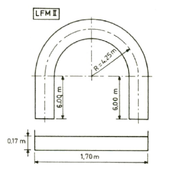
\includegraphics[width=0.5\columnwidth]{figures/testcasekalkwijkandBooij.png}
	\end{center}\caption{ A view of the case which is selected for validation purpose. It is taken from Kalkwijk and Booij (1986)-(LFM(II) channel)}
	\label{fig:testcase_kalkwijkandBooij}
\end{figure}

\paragraph*{Linked claims}
%\begin{itemize}
%	\item
the effect of secondary flow in combination with bed load transport gives almost a similar result in Delft3D Flexible Mesh compared to Delft3D4 software.
% almost the same result compare to Delft3D software. 
%\end{itemize} 
\paragraph*{Approach}
Three models have been setup: 
\begin{enumerate}
	\item specifying all the input and using D-Flow-sed-mor module of Delft3D 4.01 software.
	\item specifying all the input but using D-FLow-sed-mor module of Delft3D Flexible Mesh (structured grid).
	\item specifying all the input but using D-FLow-sed-mor module of Delft3D Flexible Mesh (unstructured grid).
\end{enumerate}

\paragraph*{Model description}
A simple structured and unstructured flexible mesh networks for the arch channel are built with the dimensions shown in \Fref{fig:testcasekalkwijkandBooij}. Curvilinear grid also generated similar to FM-net as shown in \ref{fig:FMnet}. 

\begin{figure}[h!]
	\begin{center}
		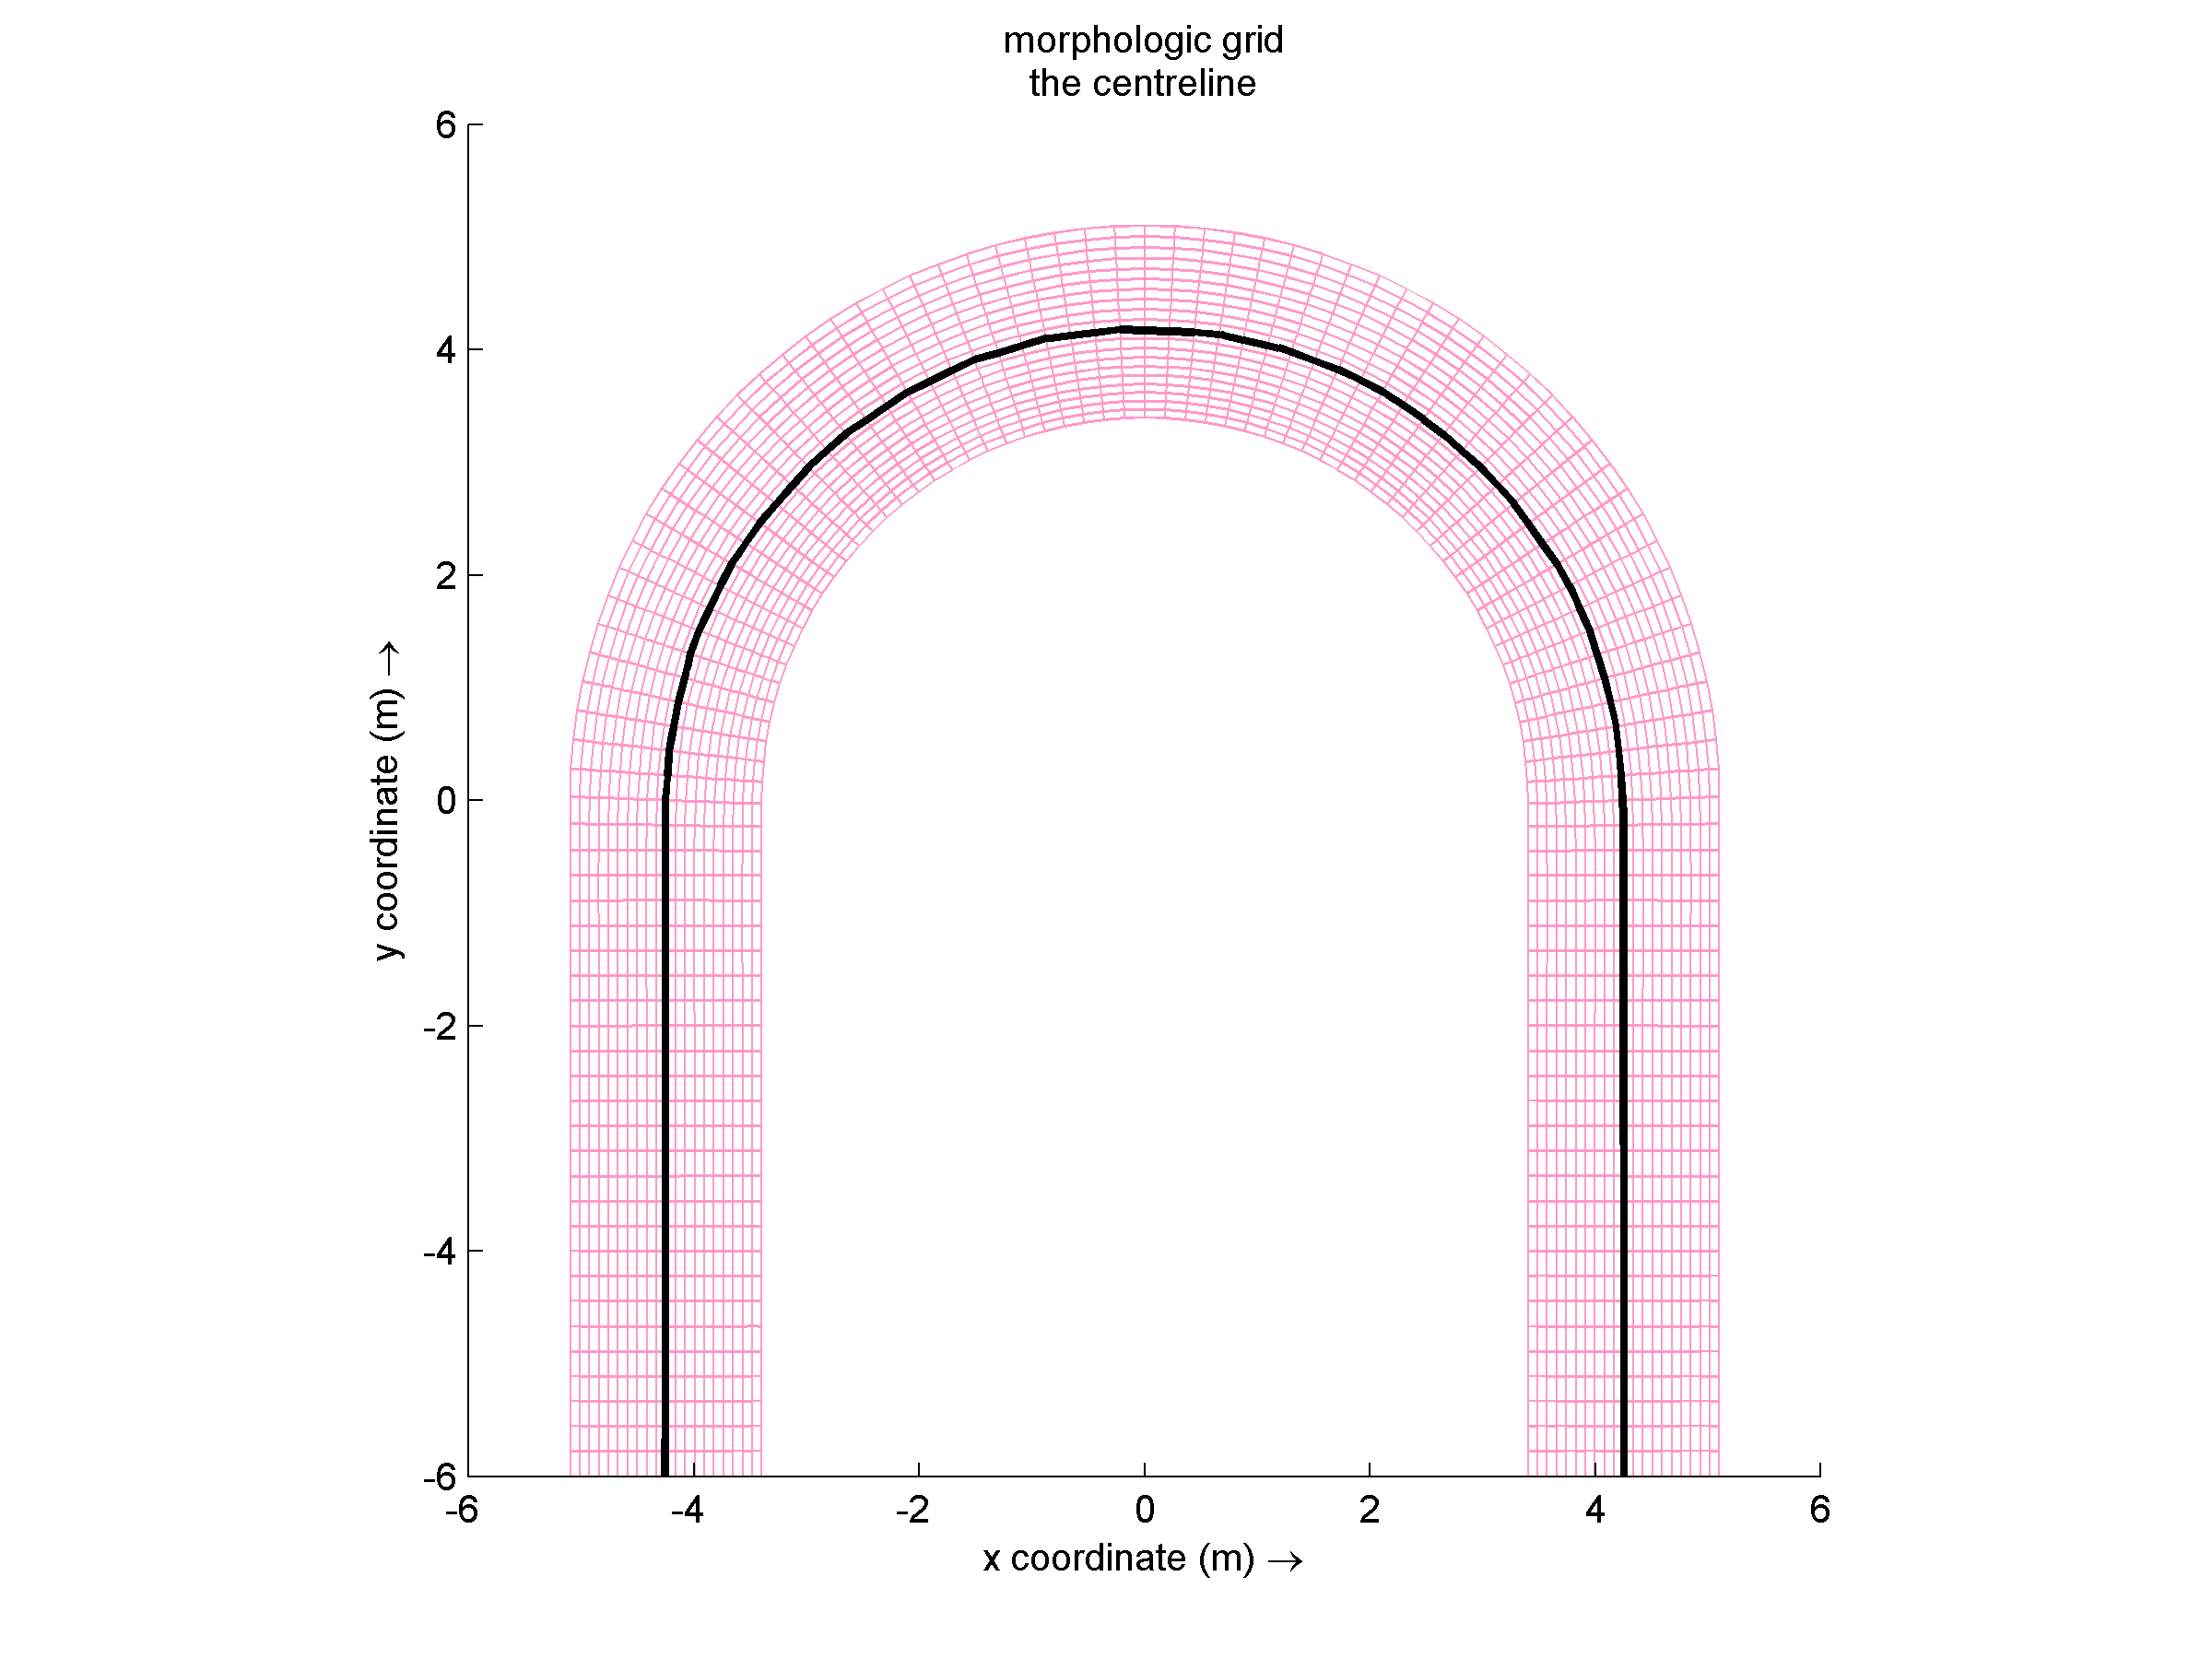
\includegraphics[width=1.0\columnwidth]{figures/FMnet.png}
	\end{center}\caption{The network used to test the coupling of secondary flow.}
	\label{fig:FMnet}
\end{figure}

\subparagraph{test-case c30 (coupling without MorUp)}
The test cases concern LFM(II) channel flow with bed level of zero and a constant roughness factor under equilibrium flow conditions. A discharge $Q$ equal to 0.5 m$^3$/s is prescribed as upstream boundary condition. The longitudinal bottom slope $i_b$ is prescribed to be $0$. The Ch\'ezy friction coefficient $C$ is set to 60 m$^{1/2}$/s. The downstream boundary condition is water level set to 0.7 m.
In addition, an important related setup to morphology file and sediment file used in these test cases are described as follows:
\begin{itemize}
	\item[$\bullet$] Sediment file <*.sed>:
\end{itemize}
\begin{verbatim}
[Sediment]
SedTyp           = bed load               # Must be "sand", "mud" or "bed load"
SedDia           = 2.0e-004               # [m] Median sediment diameter (D50)
TraFrm           = 1
Name             = #Engelund-Hansen (1967)#
ACal             = 0.6
RouKs            = 0.08
\end{verbatim}

\begin{itemize}
	\item[$\bullet$] Morphology file <*.mor>:
\end{itemize}

\begin{verbatim}
MorUpd           = False	    #	Update bathymetry during simulation 
CmpUpd           = False     # Bed composition update during simulation
ISlope	          =  3.0      # Bed slope formulation ( 3=Koch & Flokstra, 1980)
AShld            =  0.2      # [-] Bed slope parameter Koch & Flokstra
BShld            =  0.5      # [-] Bed slope parameter Koch & Flokstra
Espir            = 1         # Effect of spiral flow on bed load transport
\end{verbatim}

The bed load transport is checked too see if the direction of bed load transport is similar in FM and Delft3d. Figure \ref{fig:vic} shows the comparison of the transport direction between the three simulation. Bed load transport pattern is also illustrated in the map view of figure \ref{fig:Map}. However, the bed load magitude along the model centerline is not fully similar (compare \ref{fig:Cen}).
\begin{figure}[h!]
	\begin{center}
		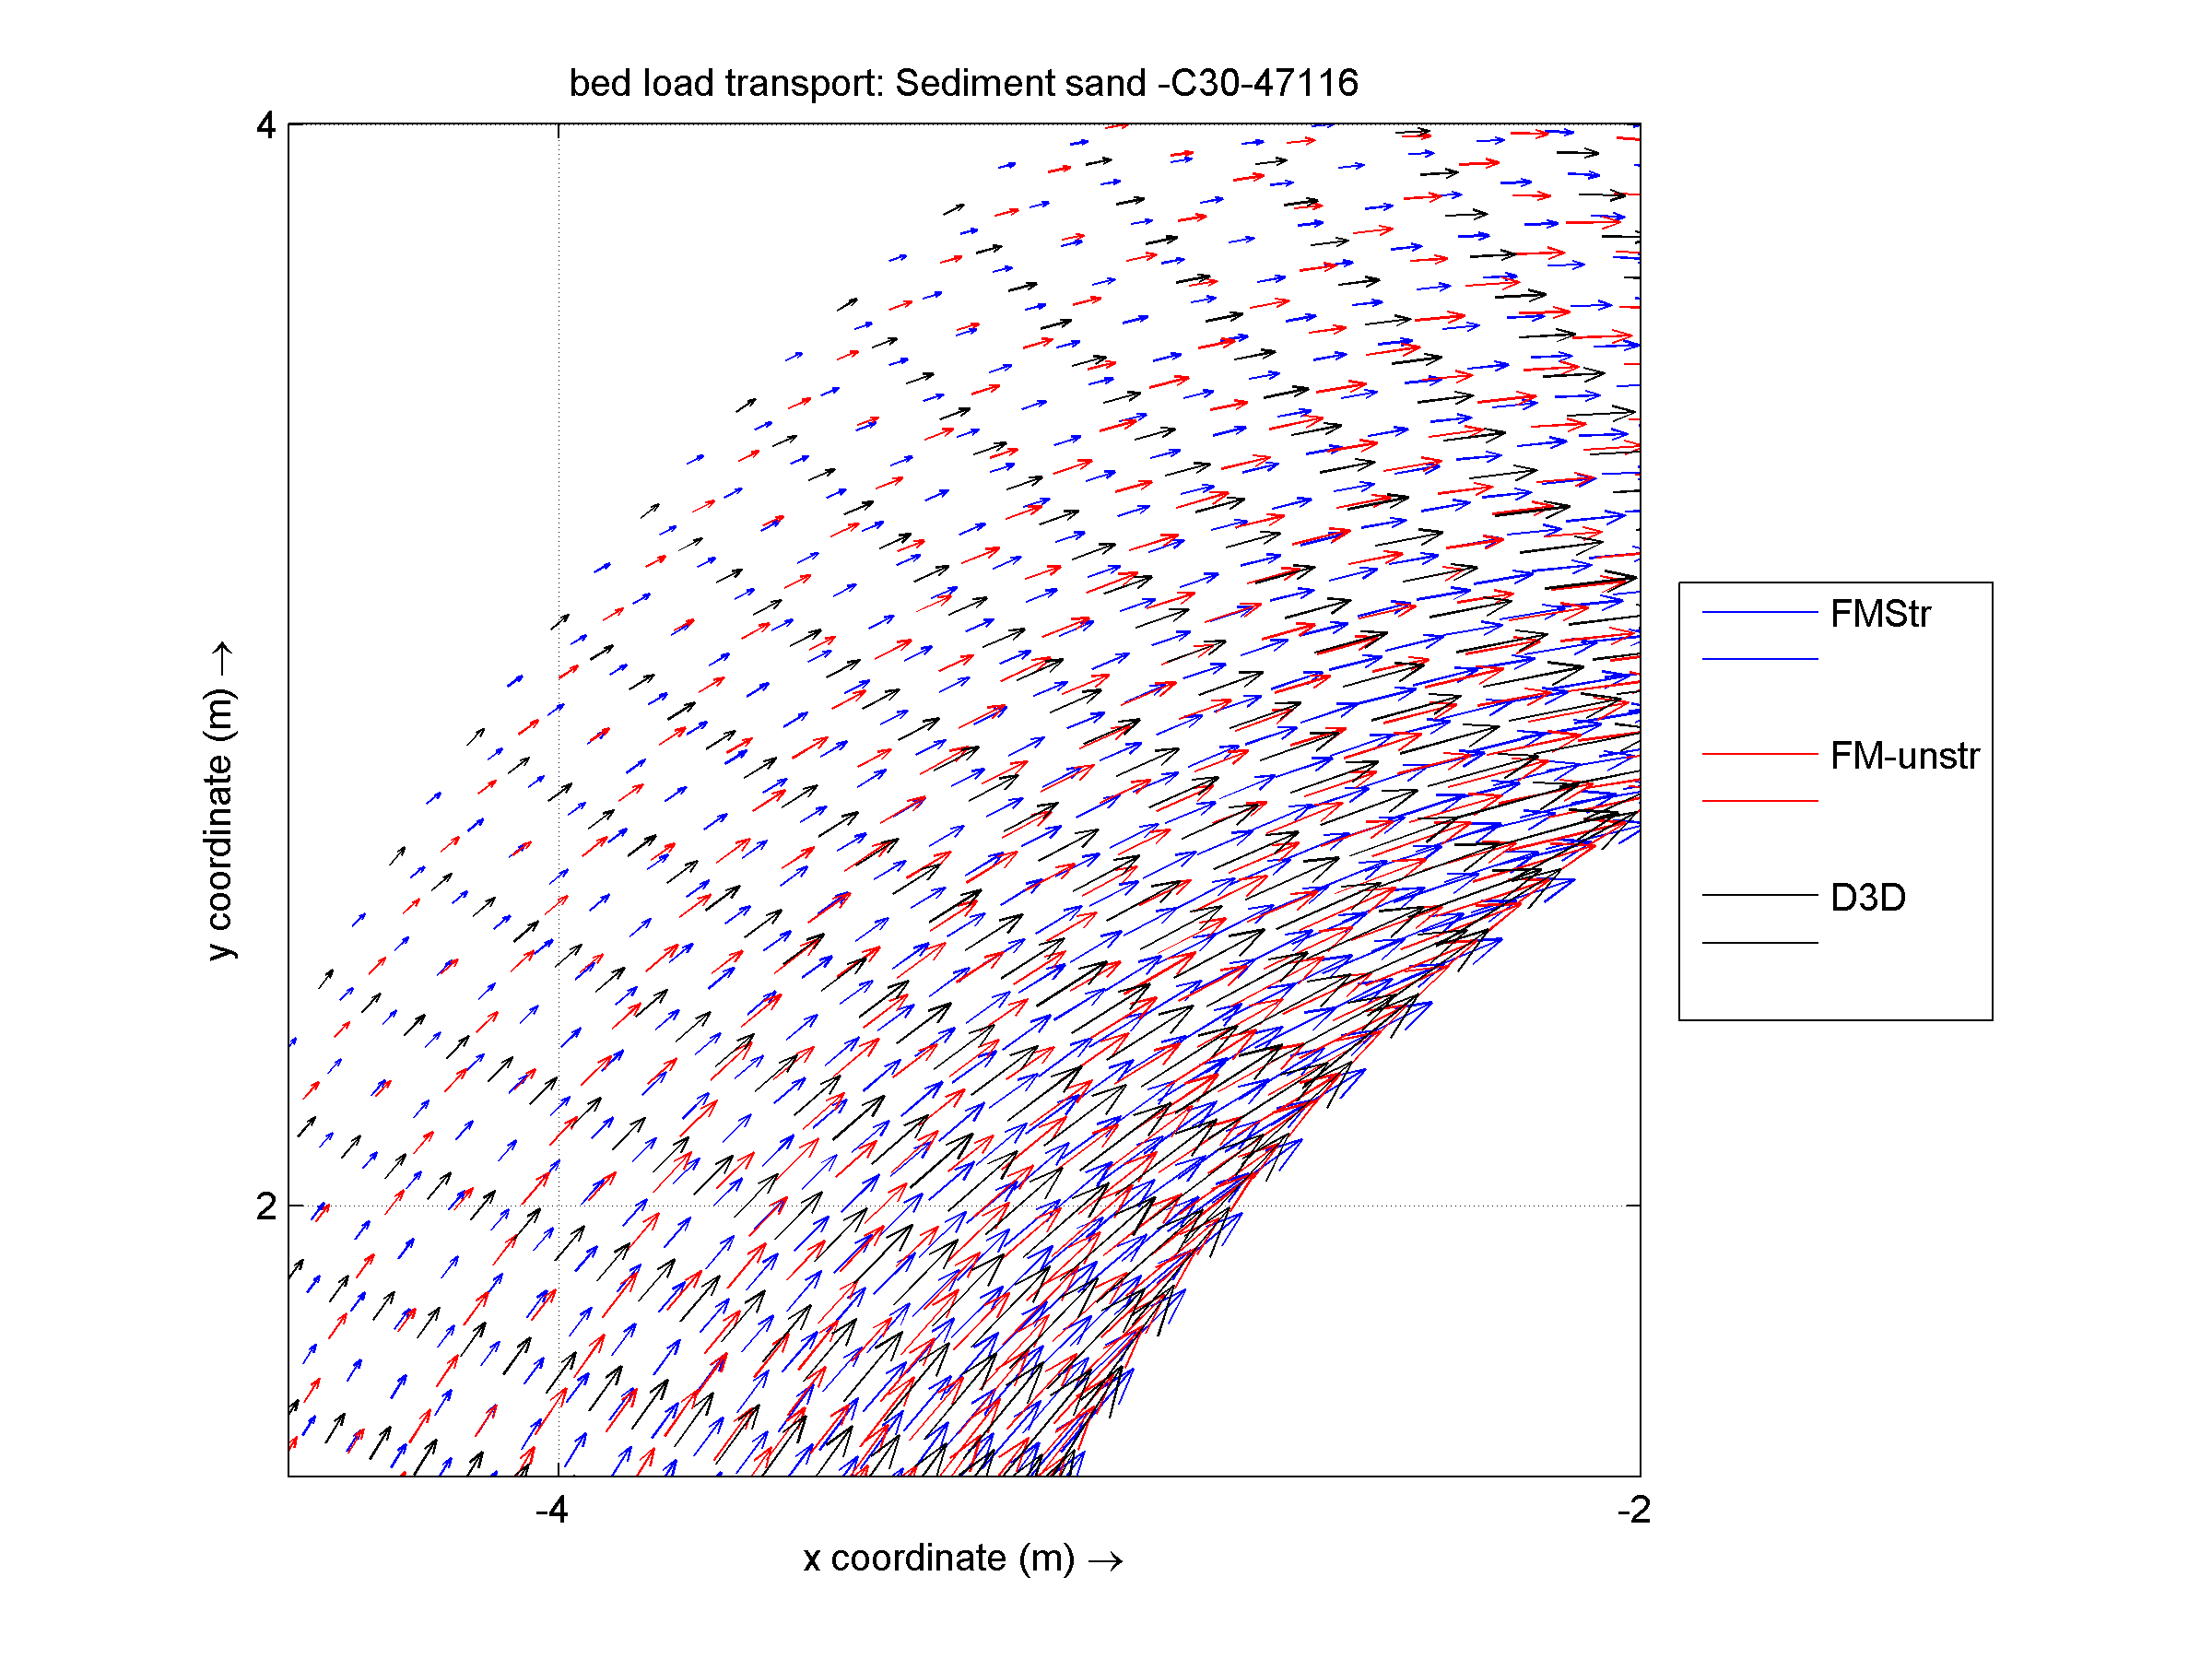
\includegraphics[width=0.7\columnwidth]{figures/C30-bedTransport2flow-VectorMap.png}
	\end{center}\caption{The direction of bed load transport at the right bend of the model domain (C30)}
	\label{fig:vic}
\end{figure}
\begin{figure}[h!]
	\begin{center}
		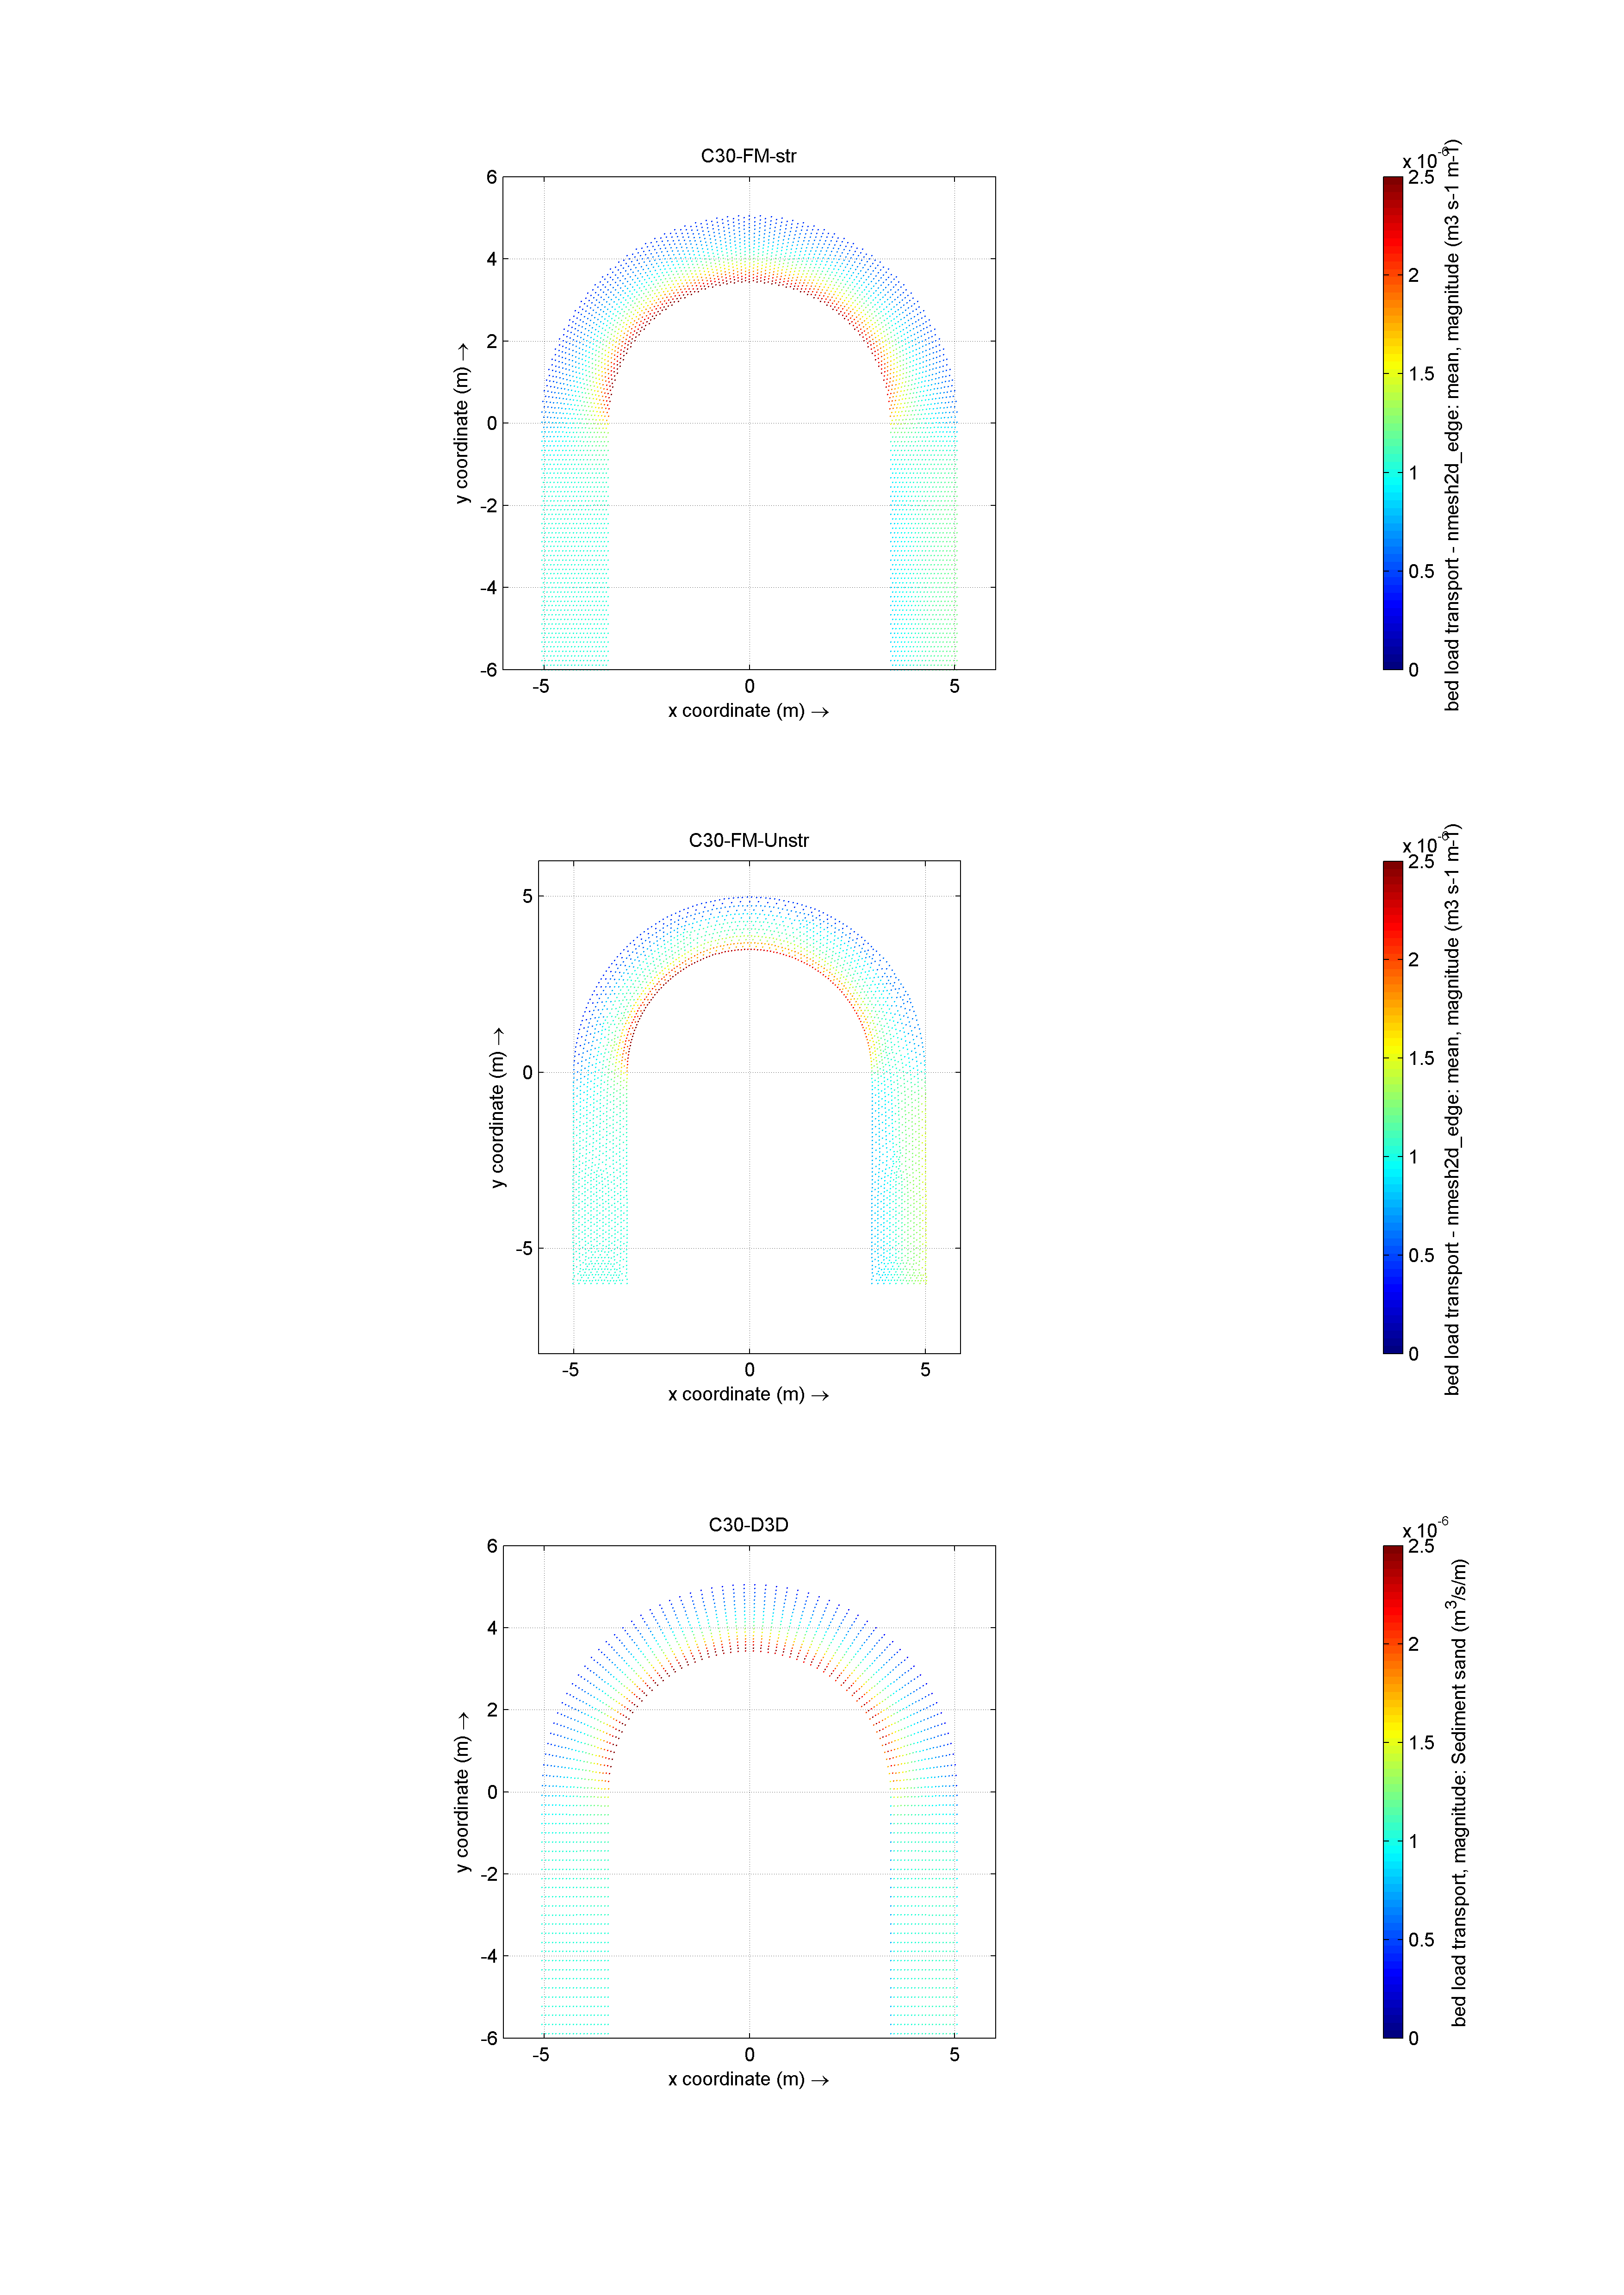
\includegraphics[width=0.7\columnwidth]{figures/C30-2flowcoupling-47116.png}
	\end{center}\caption{The bed load transport map view (c30)}
	\label{fig:Map}
\end{figure}
\begin{figure}[h!]
	\begin{center}
		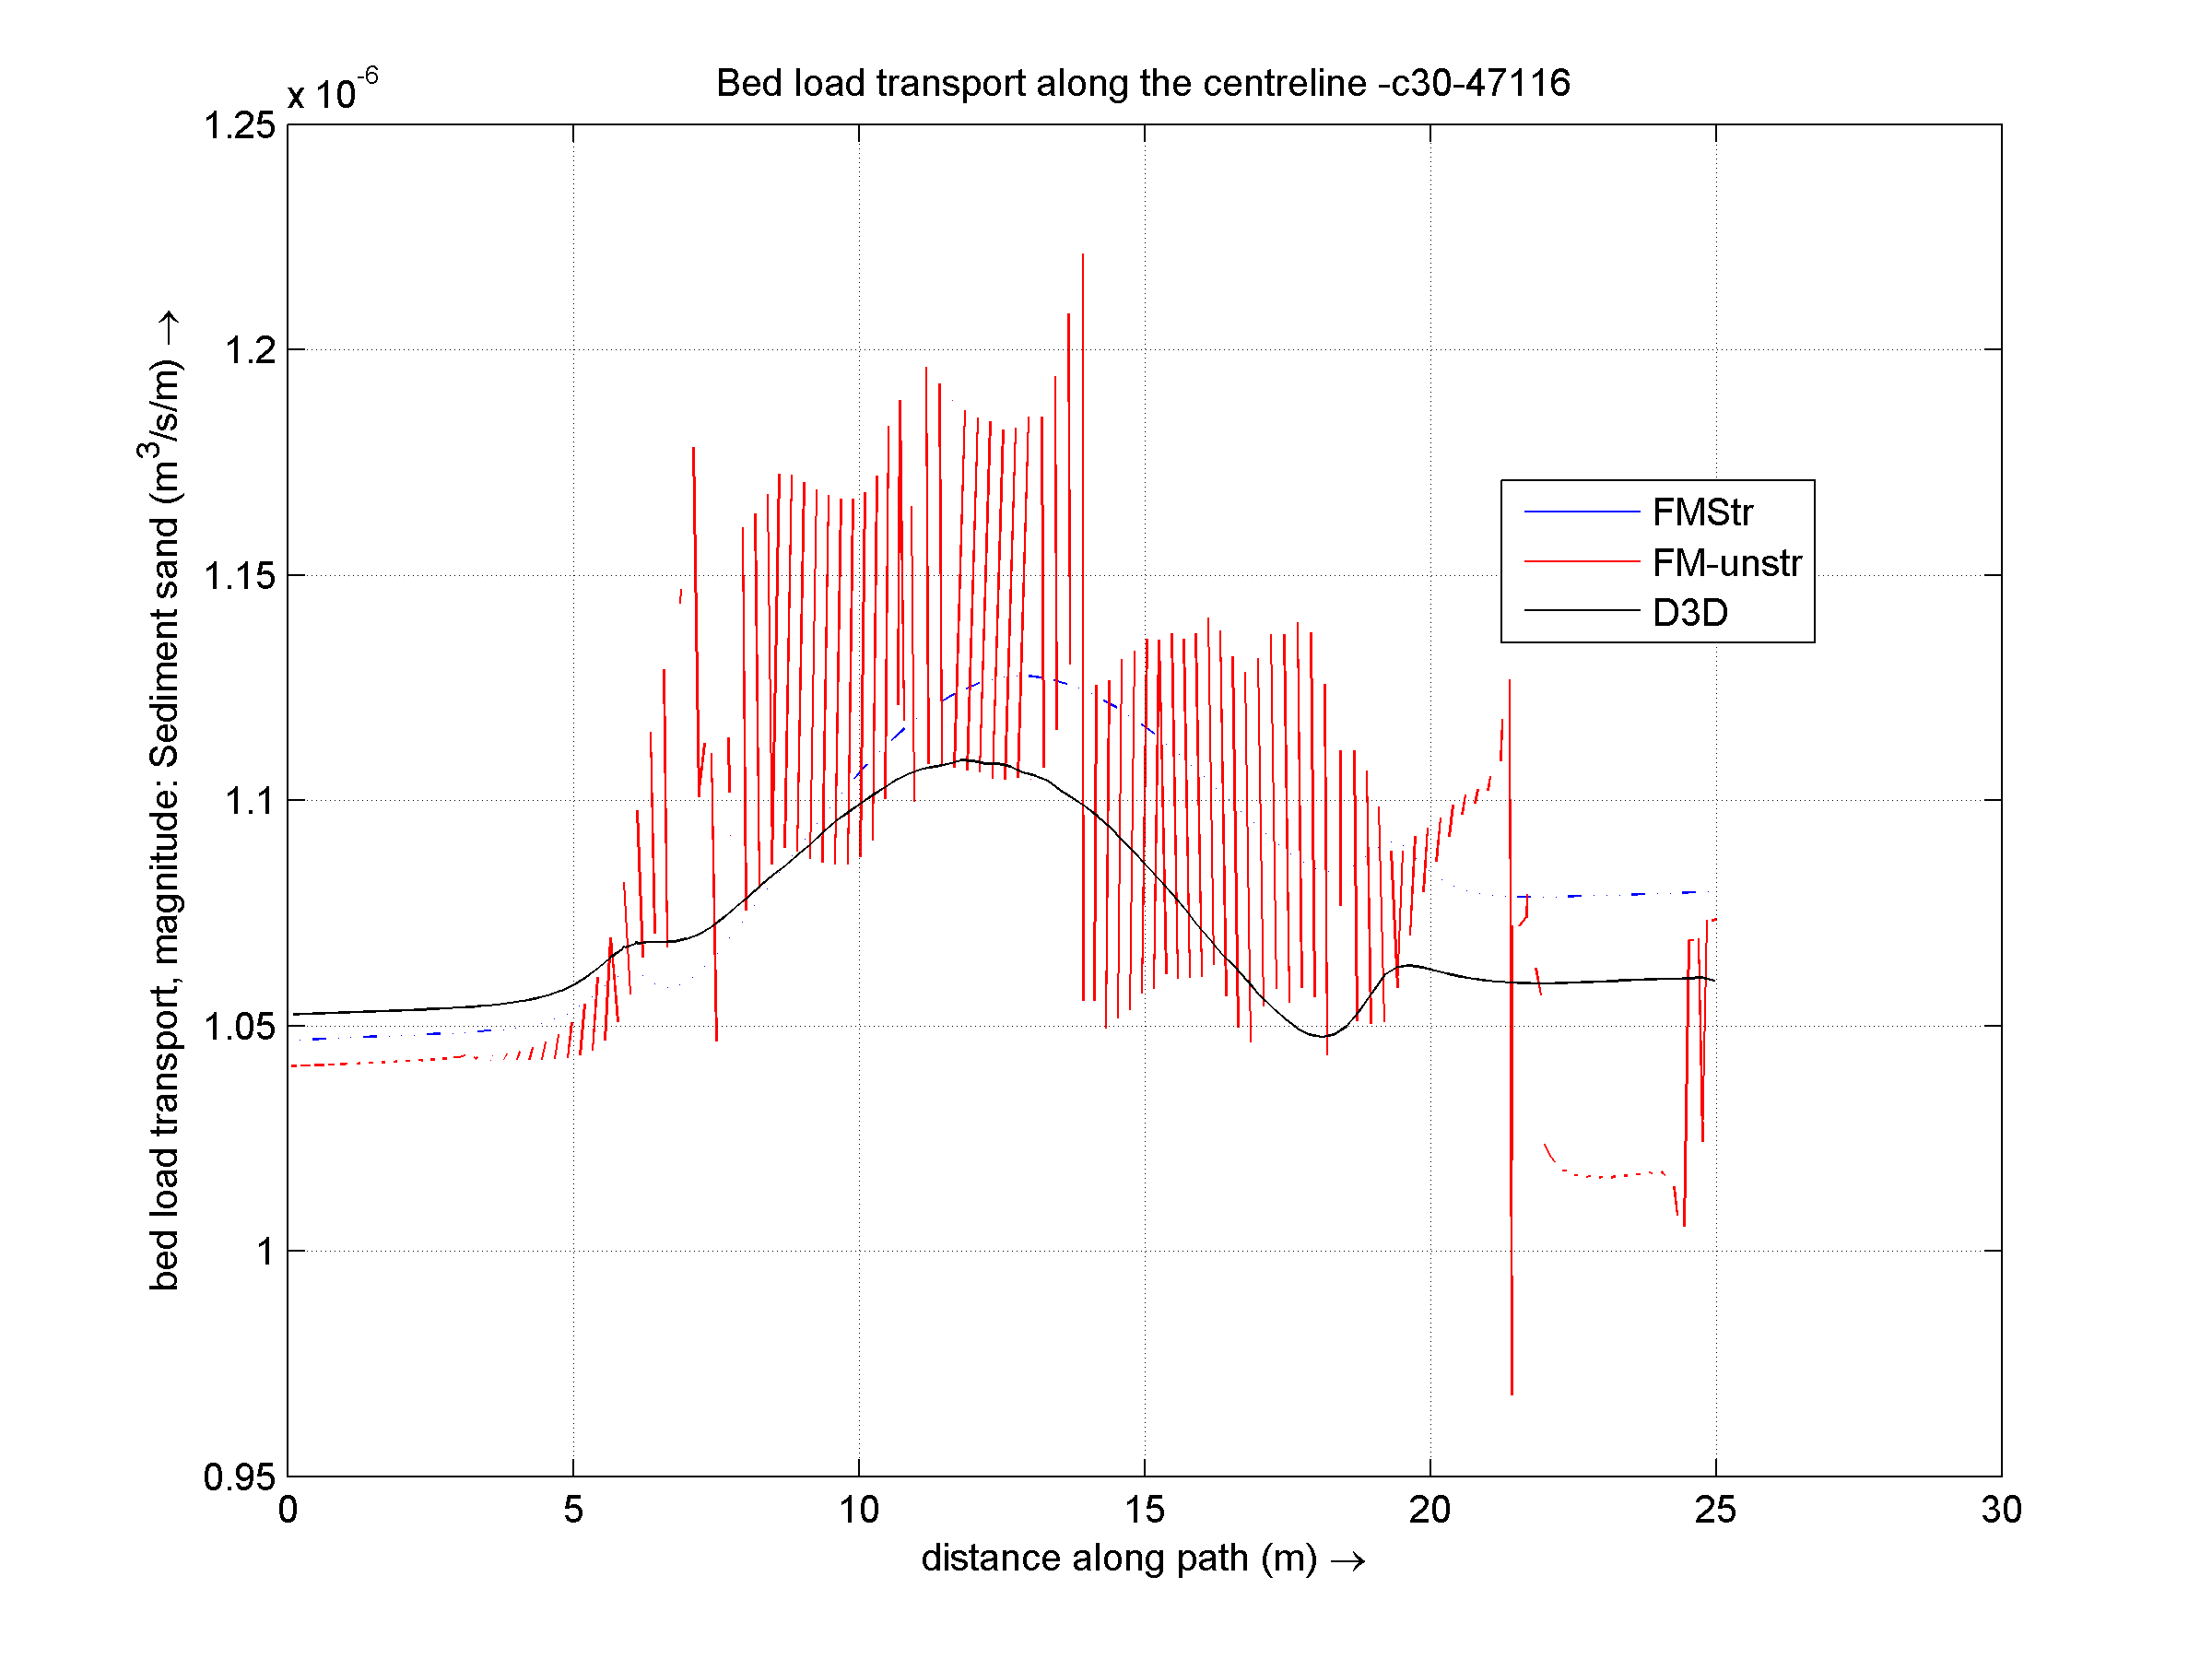
\includegraphics[width=0.7\columnwidth]{figures/C30bedtransportcentreline-47116.png}
	\end{center}\caption{Bed load transport along centerline of the model domain}
	\label{fig:Cen}
\end{figure}

\subparagraph{test-case c31 (coupling with MorUp)}
In this test case the morphological update of is switched on in the mor file to check the bed change behaviour in stuctured and unstructured grid of FM and the Delft3D4.
Figure \ref{fig:bedmap} illustrates the bed level change map of the three simulation. The trend and pattern are almost similar. However, the magnitude of bed change along the cnterline of the model show some difference in between the three simulation as shown in figure \ref{fig:cenL}.

\begin{figure}[h!]
	\begin{center}
		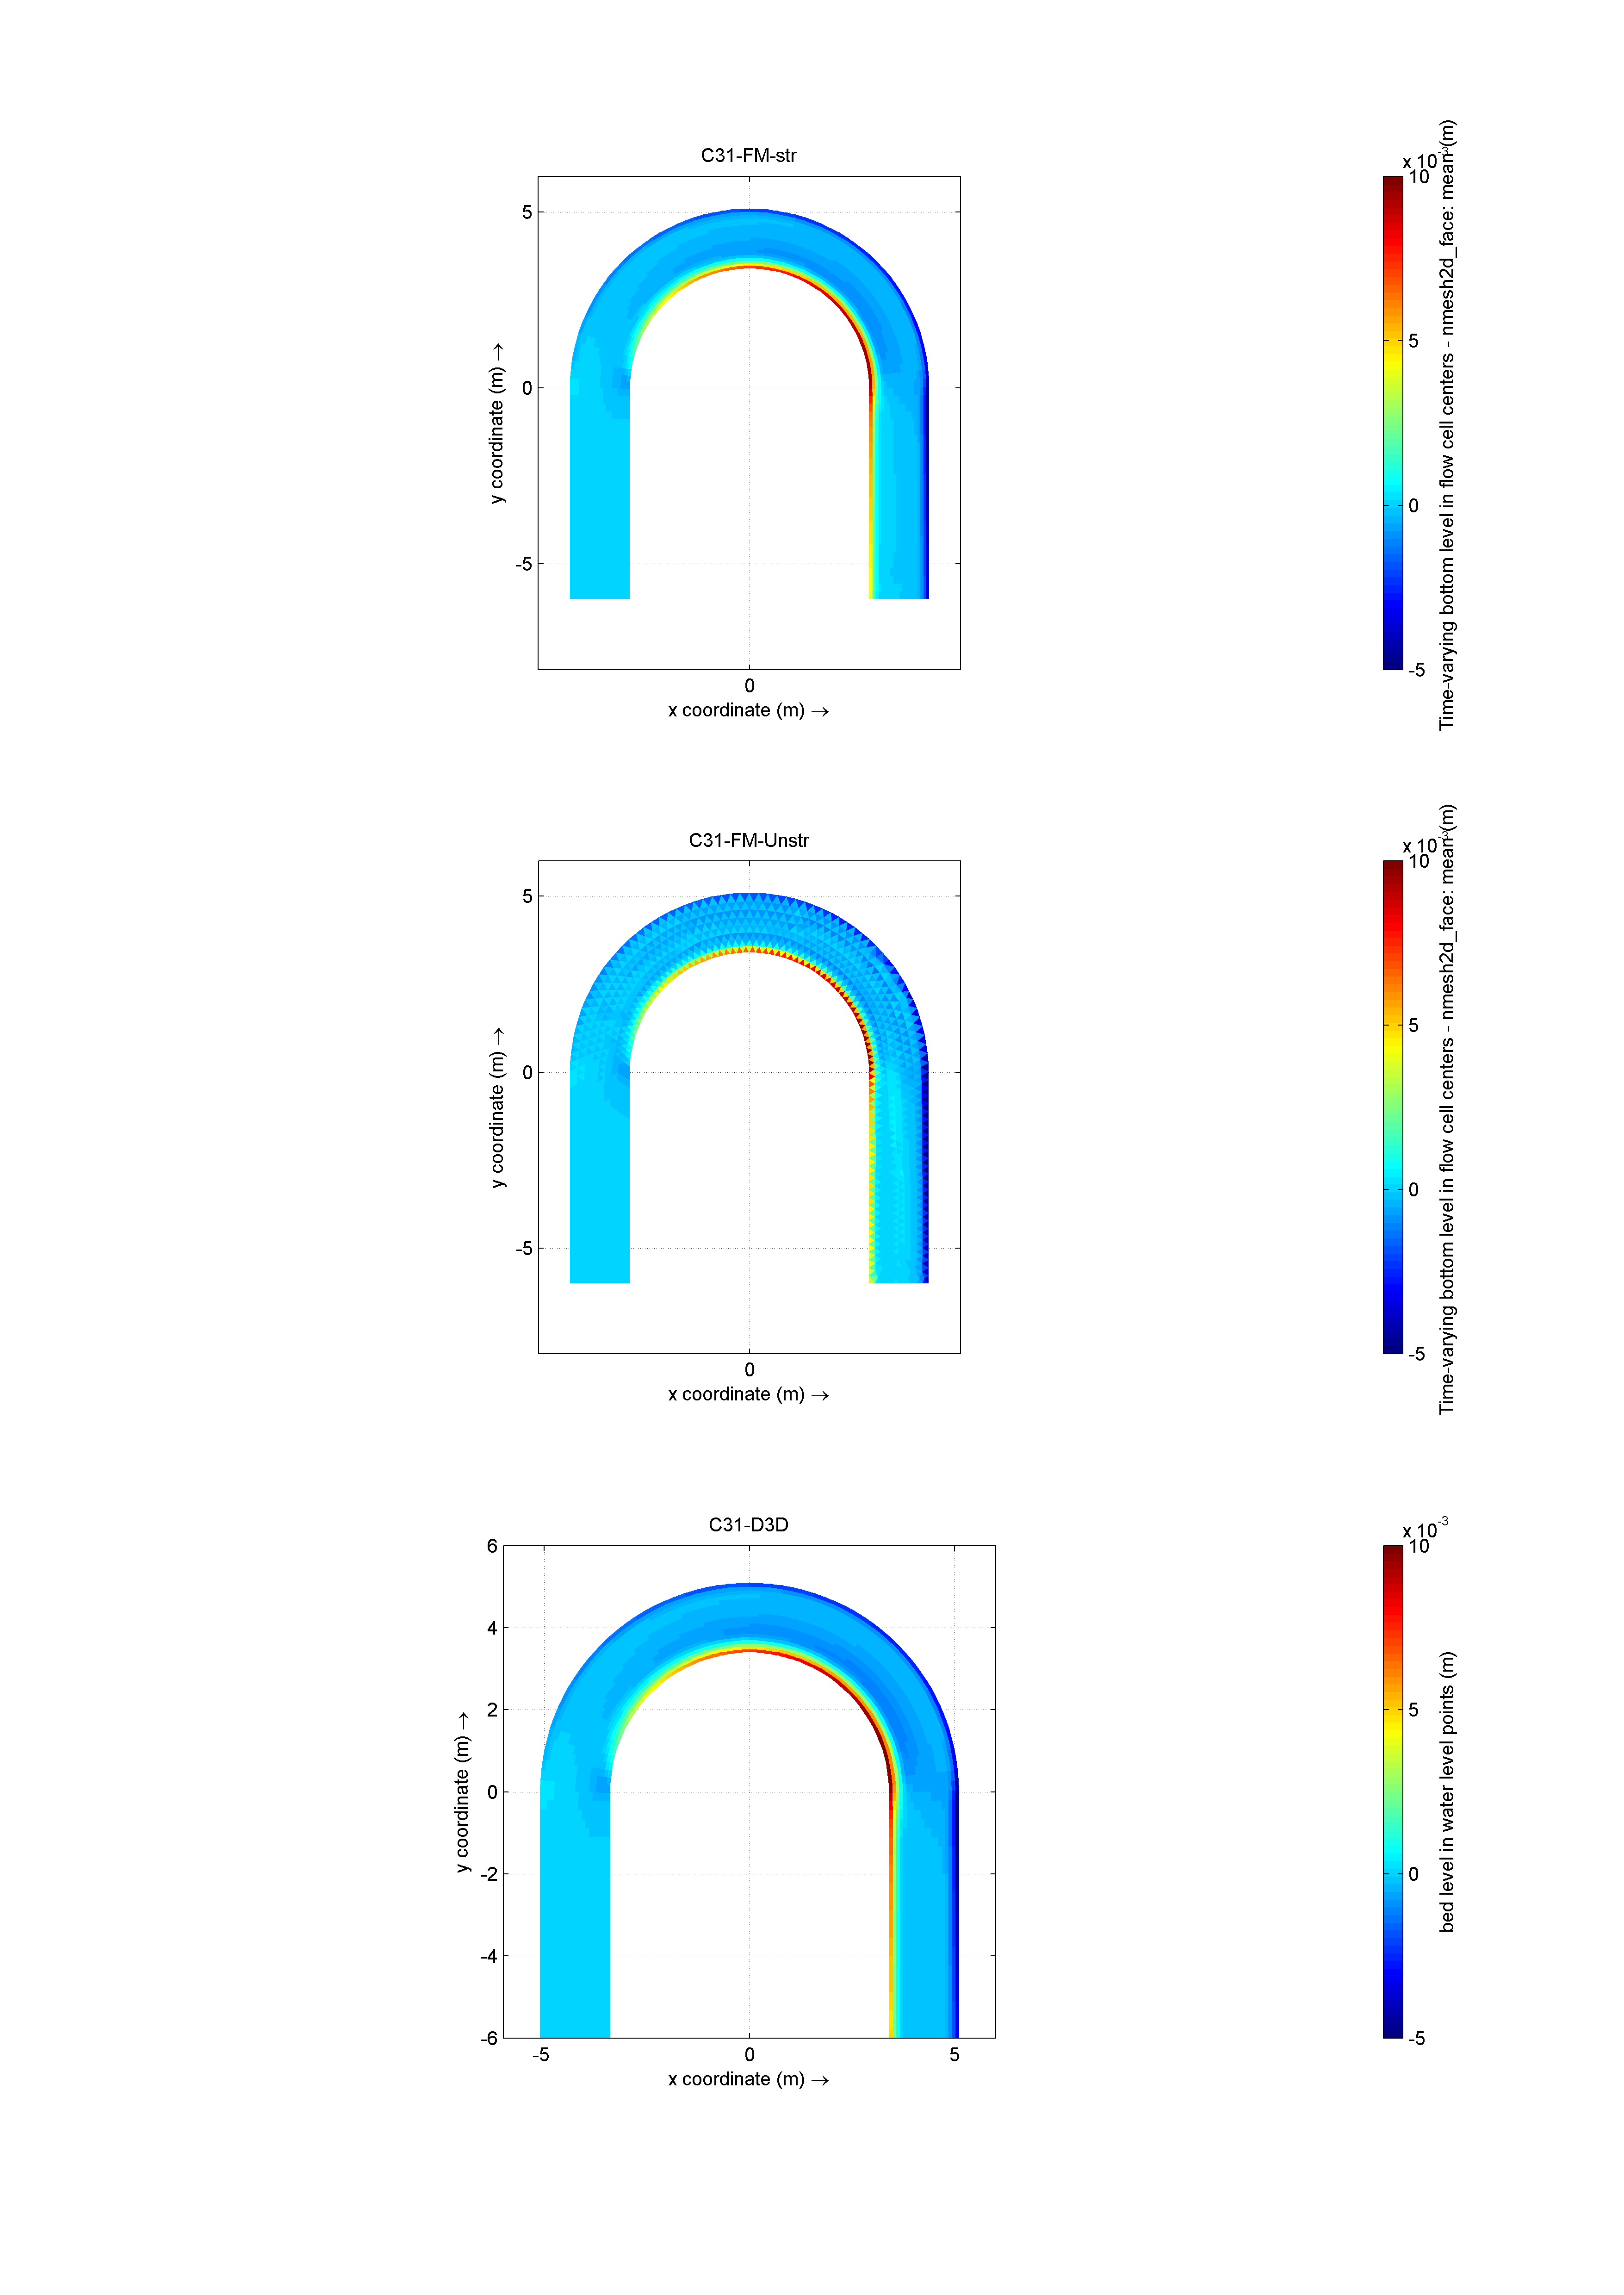
\includegraphics[width=0.7\columnwidth]{figures/C31-2flowcoupling-47116.png}
	\end{center}\caption{Bed level change map (C31)}
	\label{fig:bedmap}
\end{figure}
\begin{figure}[h!]
	\begin{center}
		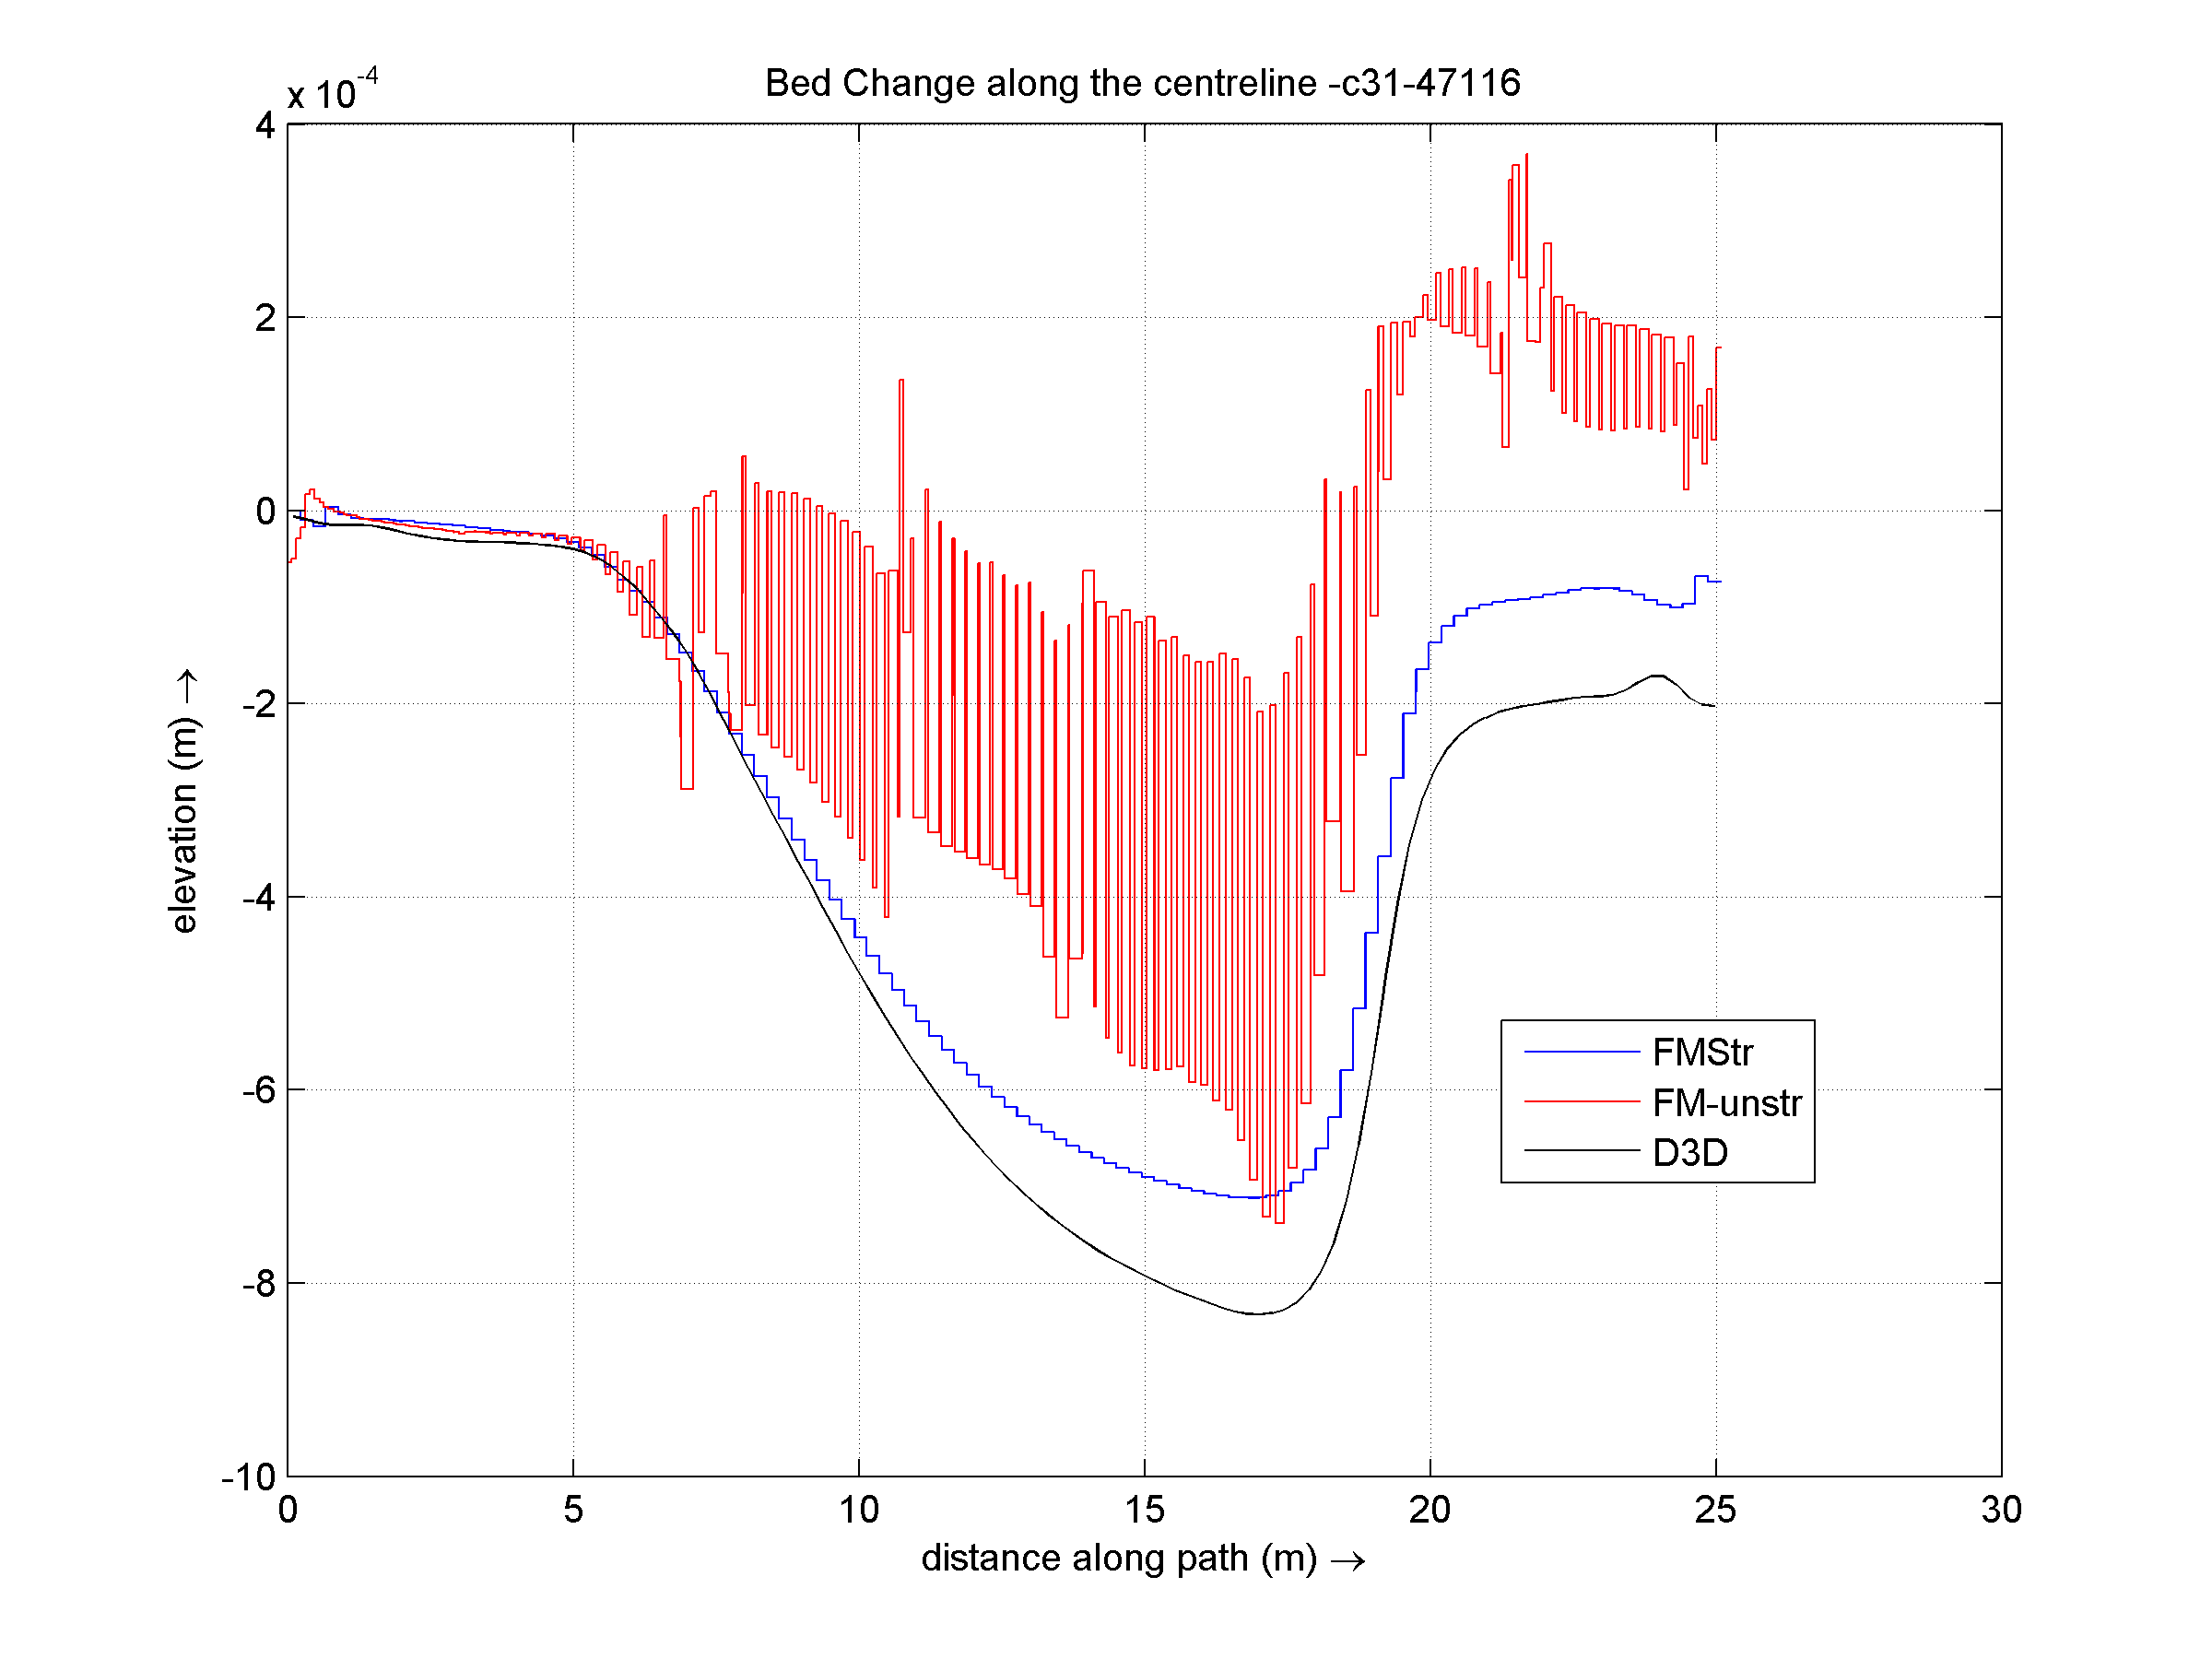
\includegraphics[width=0.7\columnwidth]{figures/C31bedChangecentreline-47116.png}
	\end{center}\caption{Bed level change magnitude along model centerline}
	\label{fig:cenL}
\end{figure}	
\paragraph*{Results}

The results show that the coupling between secondary flow and bed loadtransport gives almost similar in structured and unstructured FM net as Delft3D4 , in term of transport direction. However, the magnitude is not fully matching . Consequently, this shall be reflected in the bed level change.

\paragraph*{Conclusion}
The result shows that coupling the secondary flow with the  bed load transport and morphology works well in term of transport direction, but still further investigation is needed to match the maganitude of bed changes as the result of this test shows discrepancies.
\paragraph*{Version}
This test has been carried out using the following software versions:
\begin{itemize}
	
	\item[$\bullet$] dflow-fm-x64-1.1.188.47116 - Flexible Mesh. 
	\item[$\bullet$] FLOW2D3D Version 6.02.07.6118 - Delft3D4
	
\end{itemize}

%------------------------------------------------------------------------------

